%%%%%%%%%%%%%%%%%%%%%%%%%%%%%%%%%%%%%%%%%%%%%%%%%%%%%%%%%%%%%%%%%%%%%%%%%%%%%%%%%%%%%%%%%%%%%%%%%%%%%%%%%%%%%%%%%%%%%%%%%%%%%%%%%%%%%%%%%%%%%%%%%%%%%%%%%%%%%%%%%%%
% Written By Michael Brodskiy
% Class: Fundamentals of Electronics
% Professor: M. Onabajo
%%%%%%%%%%%%%%%%%%%%%%%%%%%%%%%%%%%%%%%%%%%%%%%%%%%%%%%%%%%%%%%%%%%%%%%%%%%%%%%%%%%%%%%%%%%%%%%%%%%%%%%%%%%%%%%%%%%%%%%%%%%%%%%%%%%%%%%%%%%%%%%%%%%%%%%%%%%%%%%%%%%

\documentclass[12pt]{article} 
\usepackage{alphalph}
\usepackage[utf8]{inputenc}
\usepackage[russian,english]{babel}
\usepackage{titling}
\usepackage{amsmath}
\usepackage{graphicx}
\usepackage{enumitem}
\usepackage{amssymb}
\usepackage[super]{nth}
\usepackage{everysel}
\usepackage{ragged2e}
\usepackage{geometry}
\usepackage{multicol}
\usepackage{fancyhdr}
\usepackage{cancel}
\usepackage{siunitx}
\usepackage{physics}
\usepackage{tikz}
\usepackage{mathdots}
\usepackage{yhmath}
\usepackage{cancel}
\usepackage{color}
\usepackage{array}
\usepackage{multirow}
\usepackage{gensymb}
\usepackage{tabularx}
\usepackage{extarrows}
\usepackage{booktabs}
\usepackage{lastpage}
\usetikzlibrary{fadings}
\usetikzlibrary{patterns}
\usetikzlibrary{shadows.blur}
\usetikzlibrary{shapes}

\geometry{top=1.0in,bottom=1.0in,left=1.0in,right=1.0in}
\newcommand{\subtitle}[1]{%
  \posttitle{%
    \par\end{center}
    \begin{center}\large#1\end{center}
    \vskip0.5em}%

}
\usepackage{hyperref}
\hypersetup{
colorlinks=true,
linkcolor=blue,
filecolor=magenta,      
urlcolor=blue,
citecolor=blue,
}


\title{Lecture 2}
\date{\today}
\author{Michael Brodskiy\\ \small Professor: M. Onabajo}

\begin{document}

\maketitle

\begin{itemize}

  \item Current-Amplifier Model

    \begin{figure}[H]
      \centering
      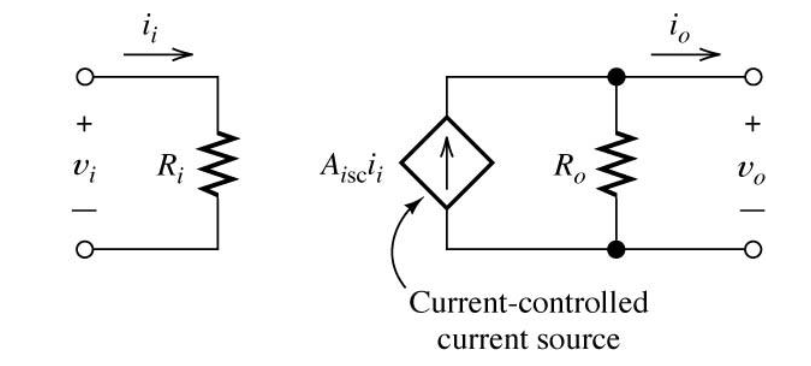
\includegraphics[width=.7\textwidth]{Images/CAM.png}
      \caption{Reference Figure for Current-Amplifier Model}
      \label{fig:1}
    \end{figure}

    \begin{itemize}

      \item Parameters

        \begin{itemize}

          \item $i_i$ is the input current, which ideally comes from a current source

          \item $R_i$ and $R_o$ are the input and output resistances, respectively

          \item $A_{isc}$ is the short-circuit current gain

        \end{itemize}

      \item Current gain with load impedance at the output: $A_i=i_o/i_i$

    \end{itemize}

  \item Application of Th\'evenin to Norton transformation

    \begin{itemize}

      \item The connection of $R_o$ is changed, but the value remains the same

    \end{itemize}

  \item $A_{isc}=i_{osc}/i_i$ is obtained with a short-circuit at the output terminals

    \begin{itemize}

      \item where: $i_{osc}=A_{vo}v_i/R_o$ and $i_i=v_i/R_i$

      \item After substituting: $A_{isc}=A_{vo}(R_i/R_o)$

    \end{itemize}

  \item Transconductance-Amplifier Model

    \begin{figure}[H]
      \centering
      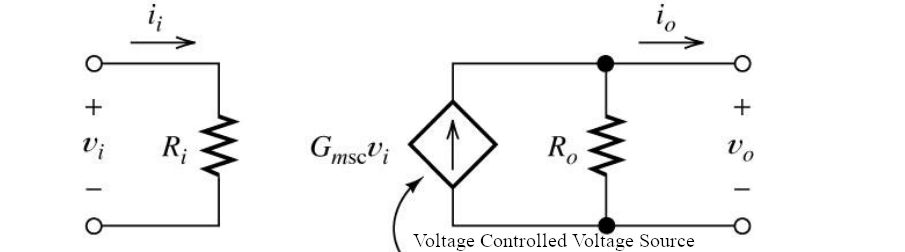
\includegraphics[width=.7\textwidth]{Images/TransConAmp.png}
      \caption{Reference Figure for Transconductance-Amplifier Model}
      \label{fig:3}
    \end{figure}

    \begin{itemize}

      \item Parameters

        \begin{itemize}

          \item $R_i$ and $R_o$ are the input and output resistances, respectively

          \item $G_{msc}$ is the short-circuit transconductance gain

        \end{itemize}

      \item Transconductance gain with load impedance: $G_m=i_o/v_i$

      \item The units of $G_{msc}$ and $G_m$ are Siemens ($S=A/V$)

      \item During model conversions: obtain $G_{msc}$ with the same short-circuit load procedure as outlined for $A_{isc}$

    \end{itemize}

  \item Transresistance-Amplifier Model

    \begin{figure}[H]
      \centering
      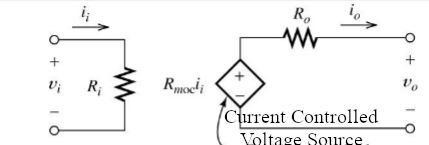
\includegraphics[width=.7\textwidth]{Images/TransResAmp.png}
      \caption{Reference Figure for Transresistance-Amplifier Model}
      \label{fig:4}
    \end{figure}

    \begin{itemize}

      \item Parameters

        \begin{itemize}

          \item $R_i$ and $R_o$ are the input and output resistances, respectively

          \item $R_{moc}$ is the open-circuit transresistance gain

        \end{itemize}

      \item Transresistance gain with load impedance: $R_m=v_o/i_i$

      \item The units of $R_{moc}$ and $R_m$ are Ohms ($\Omega$)

      \item During model conversions from Norton to Th\'evenin equivalent output stages, analyze the models with open-circuit loads:

        \begin{itemize}

          \item Transresistance-amplifier: $R_{moc}=v_{ooc}/i_i$

          \item Voltage-amplifier: $A_{vo}=v_{ooc}/v_i,\,\quad v_{ooc}\text{ is the open-circuit output voltage}$

        \end{itemize}

    \end{itemize}

  \item Conservation of Energy During Amplification

    \begin{figure}[H]
      \centering
      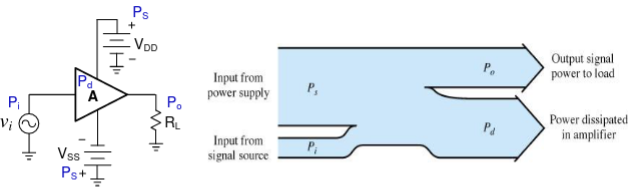
\includegraphics[width=.7\textwidth]{Images/Amps.png}
      \caption{Amplifier Energy Conservation}
      \label{fig:5}
    \end{figure}

    \begin{itemize}

      \item $P_i$ is the available power from the input signal source

      \item $P_s$ is the available power from the DC supply/supplies

      \item $P_o$ is the output power delivered to the load

      \item $P_d$ is the power dissipated in the amplifier (loss)

        $$P_i+P_s=P_o+P_d$$

      \item Amplifier efficiency:

        $$\eta=\frac{P_o}{P_s}\cdot100\%$$

    \end{itemize}

  \item Note: for input/output power calculations, RMS values must always be used

  \item Differential Amplification

    \begin{figure}[H]
      \centering
      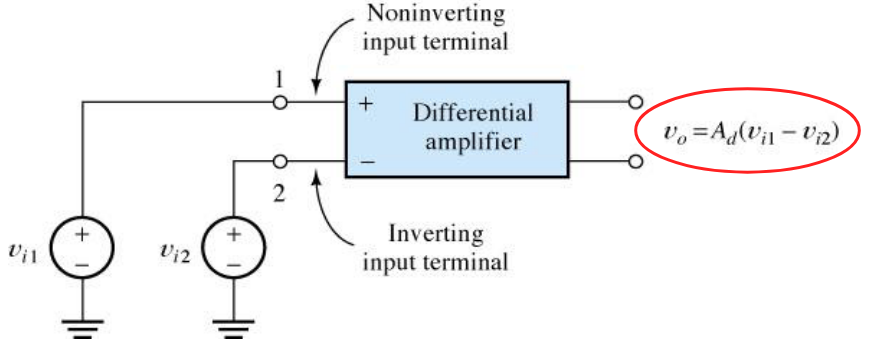
\includegraphics[width=.7\textwidth]{Images/DiffAmp.png}
      \caption{Differential Amplifier Model}
      \label{fig:6}
    \end{figure}

    \begin{itemize}

      \item Differential input signal: $v_{id}=v_{i1}-v_{i2}$

      \item Differential voltage gain: $A_d$

      \item $v_o=A_dv_{id}$

      \item Common-mode (average) input signal: $v_{icm}=\frac{1}{2}(v_{i1}+v_{i2})$

        \item Output in the presence of differential and common-mode input signals

          \begin{itemize}

            \item $v_o=A_dv_{id}+A_{cm}v_{cm}$, where $A_{cm}$ is the common-mode gain

            \item In many applications, we want: $A_{cm}=0$ (ideal case) or $A_{cm}<<A_d$

          \end{itemize}

    \end{itemize}

  \item Common-Mode Rejection

    \begin{figure}[H]
      \centering
      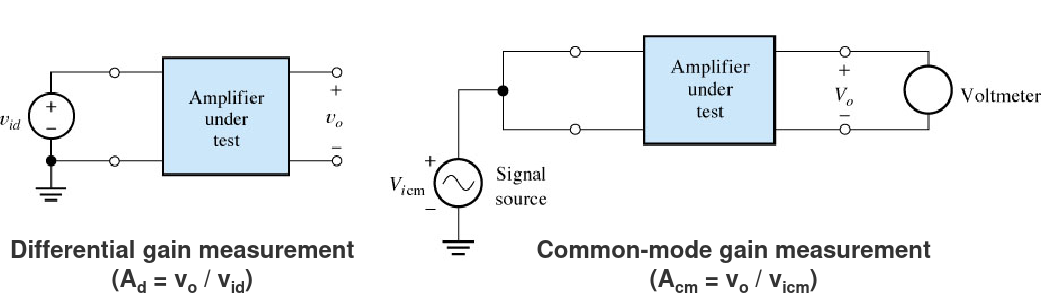
\includegraphics[width=.7\textwidth]{Images/CMRR.png}
      \caption{Common-Mode Rejection Calculation}
      \label{fig:6}
    \end{figure}

    \begin{itemize}

      \item Common-mode rejection ratio (CMRR) in decibels:

        $$CMRR=20\log\left( \frac{A_d}{A_{cm}} \right)$$

        \begin{itemize}

          \item Indicates the capacity of the amplifier to attenuate the common-mode input signal relative to the differential input signal

          \item In many applications, a high CMRR is desired $\to$ \textit{i}.\textit{e}., the amplifier rejects (reduces) the common-mode input signal components

        \end{itemize}

    \end{itemize}

\end{itemize}

\end{document}

